\chapter{Adaptación GPU}


\section{Implementación de convoluciones como GEMM \label{Intro_GEMMM}}

\begin{figure}[H]
	\centering
	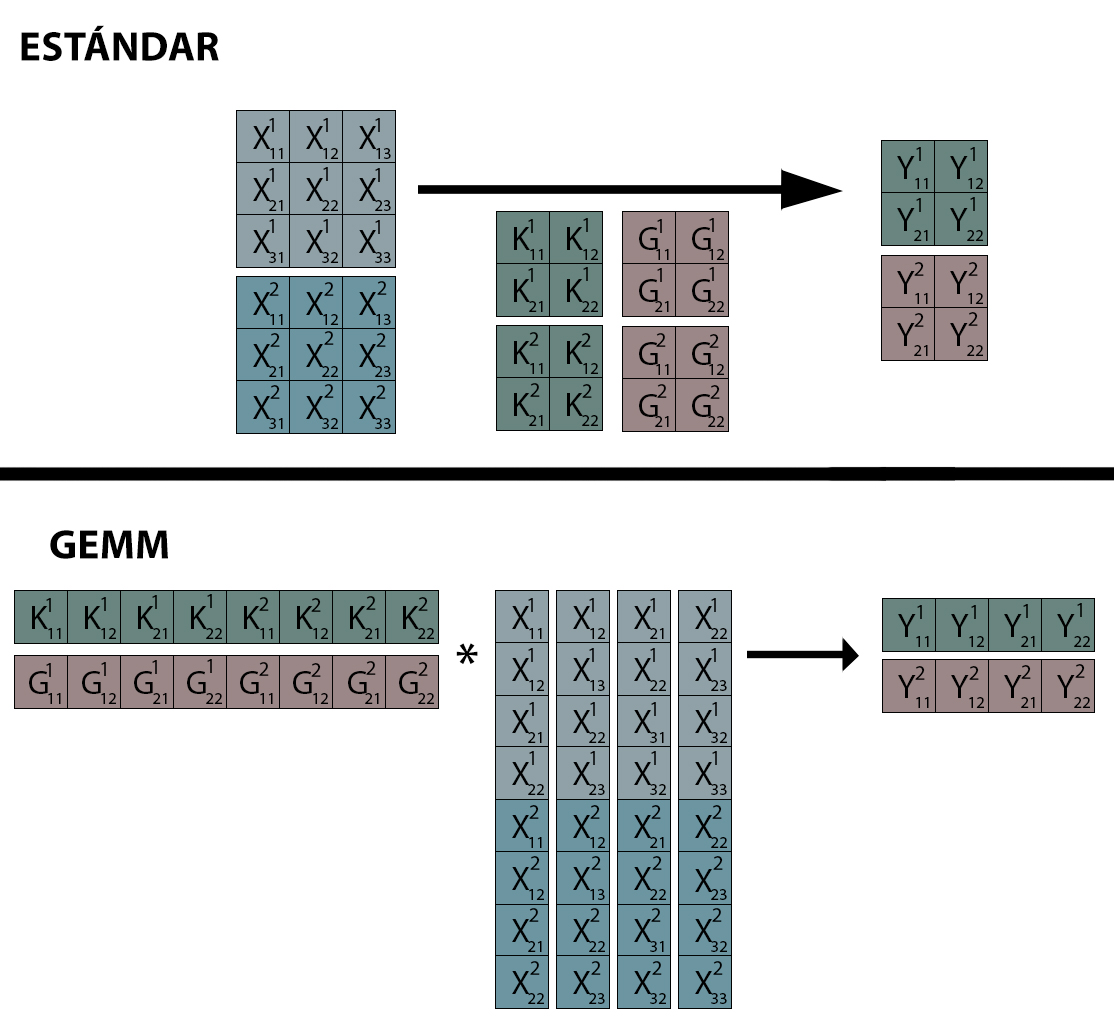
\includegraphics[scale=0.35]{imagenes/conv_std_vs_gemm.jpg}  
	\caption{Imagen de una convolución estándar frente a una convolución empleando GEMM}
	\label{fig:conv_std_vs_gemm}
\end{figure}
Se trata de un enfoque ampliamente conocido en el mundo de deep learning, empleándolo gran cantidad de librerías del sector como Caffe, Torch-cunn, Theano-CorrMM, o incluso CuDNN. \cite{conv_GEMM_FFT_comparacion} \\
GEMM permite reducir el tiempo de cómputo requerido en una convolución a cambio de aumentar el espacio necesario para la misma. Este método consiste en ``desenrrollar'' tanto el volumen de entrada X como la matriz de filtros K, además de una serie de duplicaciones de X, de tal forma que cada columna de este nuevo volumen X\_unroll contenga todos los elementos de X implicados en el cálculo de una posición distinta del volumen de salida Y. \\
En la figura \ref{fig:conv_std_vs_gemm} se muestra una comparativa visual entre una convolución implementada de forma ``estándar'' frente a una con GEMM. \\
Mientras que el método estándar requiere de varias iteraciones para calcular cada valor del volumen de salida Y (figura \ref{fig:forward_prop_convolucional}), la alternativa que presenta GEMM permite que cada valor sea el resultado de multiplicar una fila de pesos (K o G en la figura \ref{fig:conv_std_vs_gemm}) por una columna de X\_unroll. \cite{Programming_Massively} \\
De esta forma, con N kernels de tamaño KxK, un volumen de entrada con C canales de profundidad, y un volumen de salida de dimensiones $NxH_{out}xW_{out}$, una multiplicación matricial entre la matriz de pesos $M_1$ con N filas y $K^2*C$ columnas, y X\_unroll con $K^2*C$ filas y $H_{out}*W_{out}$ columnas, produce el mismo volumen de salida Y que una convolución ordinaria con N kernels distintos. \\
Por último, aunque se haya omitido para simplificar la comprensión del método planteado, tras realizar dicha multiplicación matricial se debe sumar el sesgo y aplicar la función de activación correspondiente a cada elemento del volumen de salida Y.

\subsection{Paso de capa convolucional a capa de agrupación}

\begin{figure}[H]
	\centering
	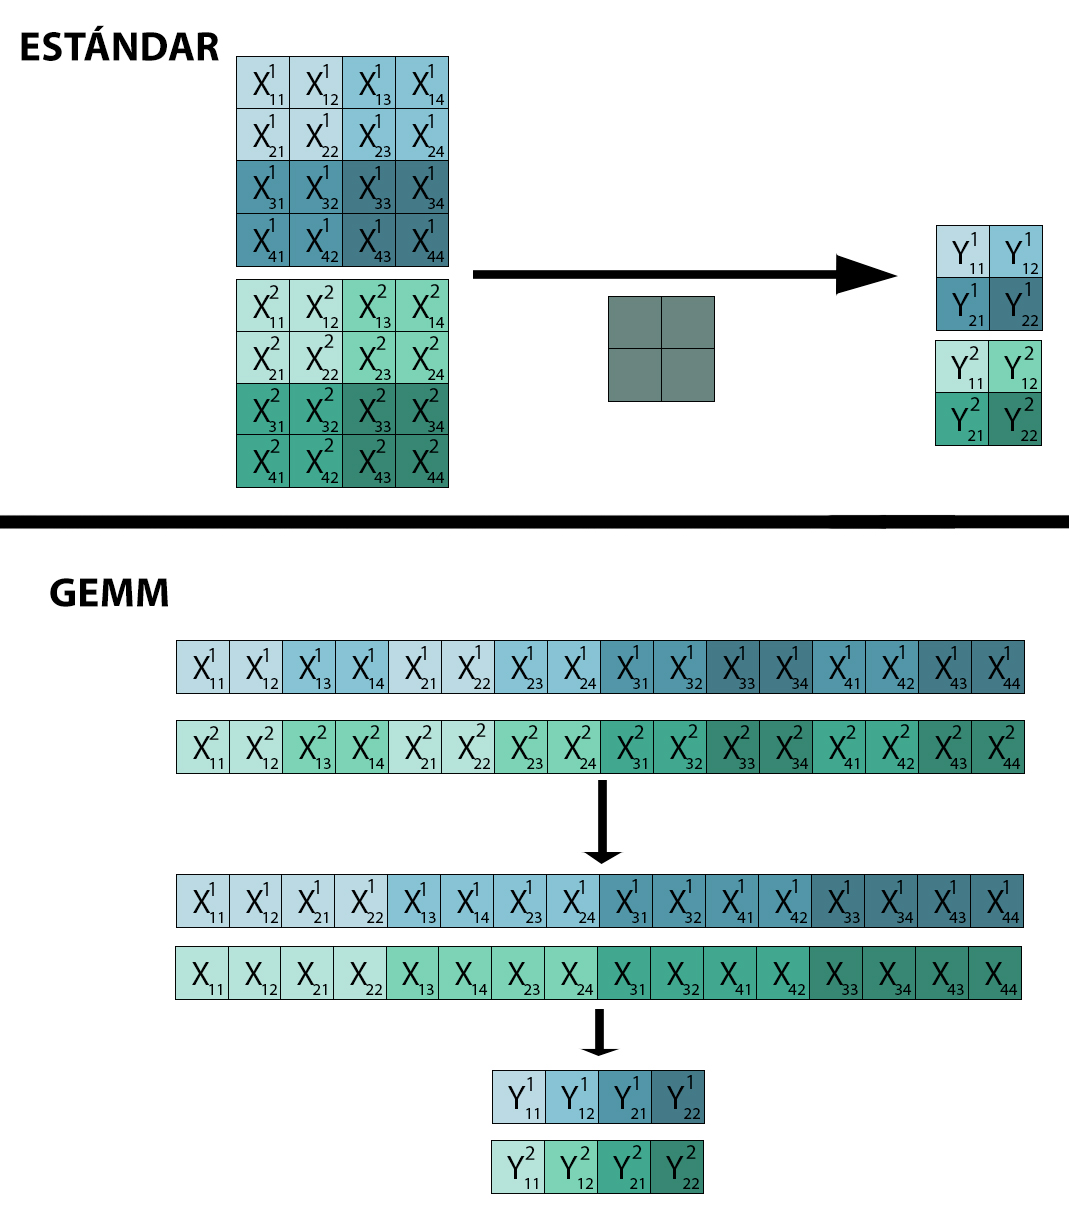
\includegraphics[scale=0.35]{imagenes/maxpool_std_vs_gemm.jpg}  
	\caption{Imagen de una agrupación con una entrada estándar frente a una agrupación con una entrada procedente de GEMM}
	\label{fig:maxpool_std_vs_gemm}
\end{figure}

\section{Retropropagación en capa convolucional con enfoque GEMM}

En la figura \ref{fig:conv_backprop_como_convolucion_Y_K_pad} se vio como la retropropagación respecto a la entrada en una capa convolucional consistía en una convolución entre los kernels de pesos y el volumen de salida. Del mismo modo, en la figura \ref{fig:conv_backprop_como_convolucion_Xpad_Y} también se mostró como el gradiente respecto a los pesos consistía en una convolución entre el volumen de entrada y el de salida. \\
Como ambos gradientes se pueden implementar como convoluciones, y en la sección \ref{Intro_GEMMM} se mostró como implementar convoluciones con el enfoque GEMM, la retropropagación en una capa convolucional se puede implementar mediante el enfoque GEMM.

\begin{figure}[H]
	\hspace{-25mm}
	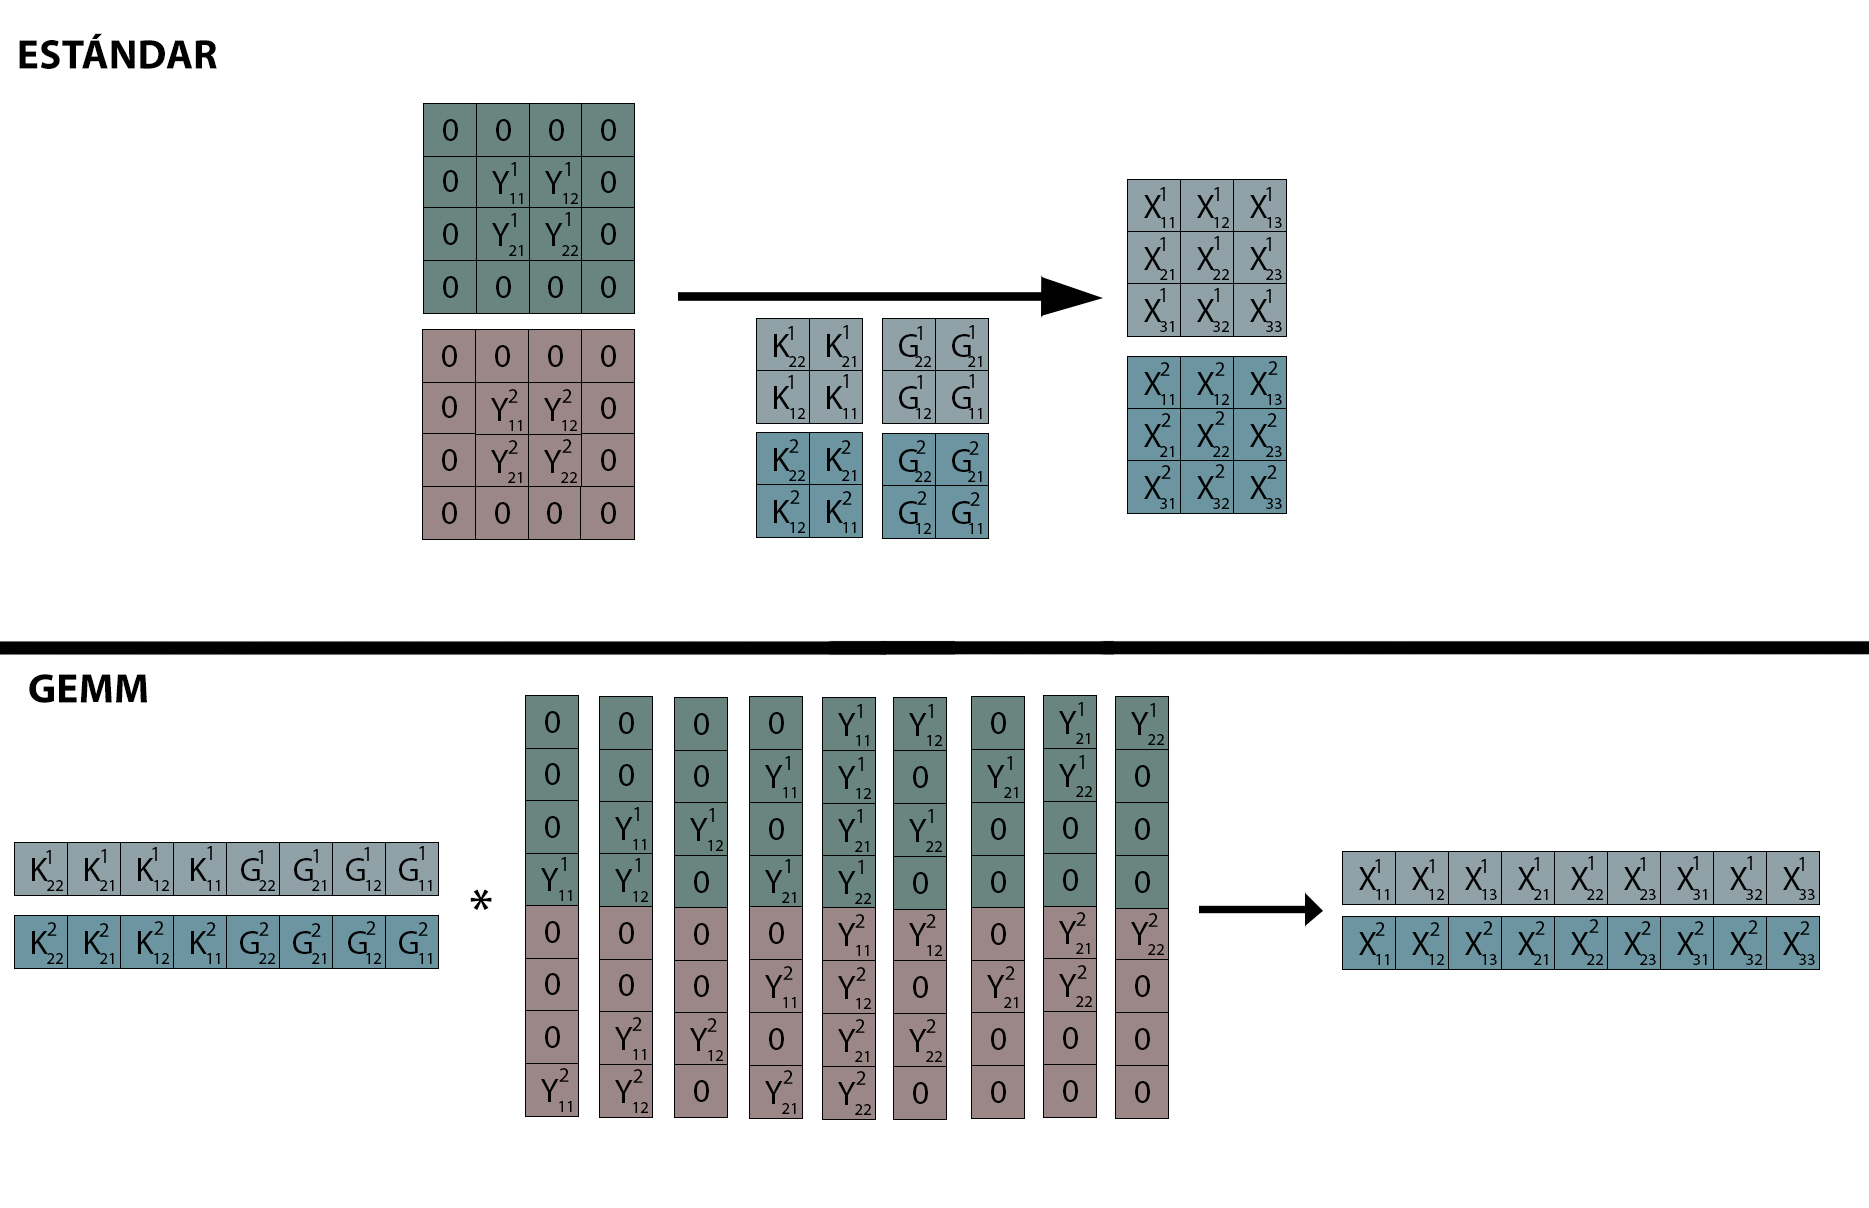
\includegraphics[scale=0.3]{imagenes/conv_std_vs_gemm_backprop.jpg}  
	\caption{Retropropagación en una capa convolucional de forma estándar frente a GEMM respecto a la entrada}
	\label{fig:conv_std_vs_gemm_backprop}
\end{figure}

\begin{figure}[H]
	\hspace{-25mm}
	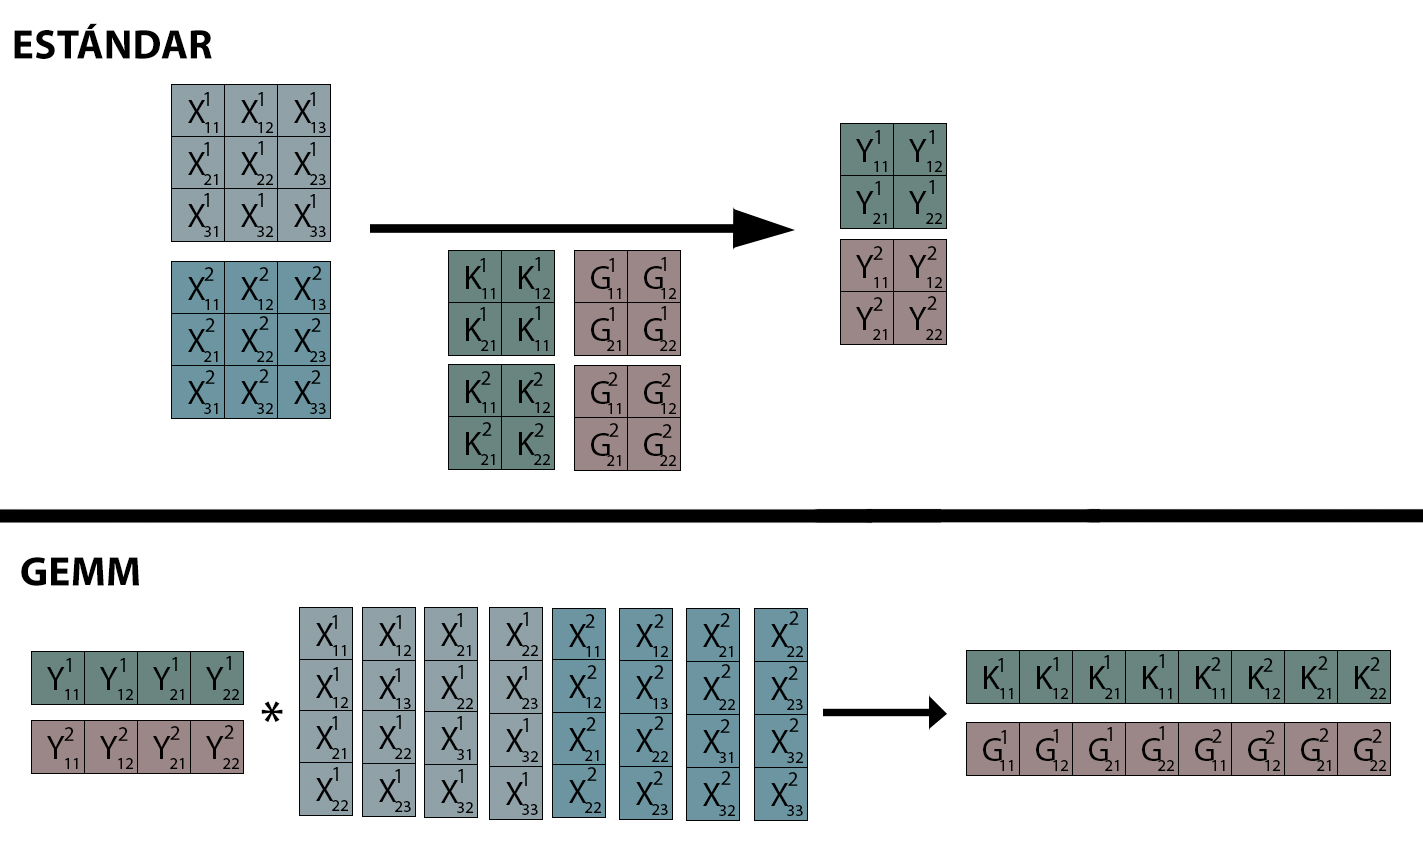
\includegraphics[scale=0.3]{imagenes/conv_std_vs_gemm_backprop_pesos.jpg}  
	\caption{Retropropagación en una capa convolucional de forma estándar frente a GEMM respecto a los pesos}
	\label{fig:conv_std_vs_gemm_backprop_pesos}
\end{figure}
